\documentclass [titlepage,a4paper]{article}

\usepackage[utf8]{inputenc}
\usepackage{makeidx}
\usepackage{graphicx}
\graphicspath{{figures/}}
\usepackage{amsmath}
\usepackage{theorem}
\usepackage[german]{babel}
\usepackage{cite}
\usepackage{textcomp}
\usepackage{fancyhdr}
\usepackage{float}
\usepackage{listings}
\usepackage{subcaption}
\fancyhead{}
\fancyhead[LO]{\bfseries \rightmark}
\fancyfoot[LO]{\thepage}
\fancyfoot[CO]{}
\pagestyle{fancy}
\bibliographystyle{ieeetr}
\usepackage[title]{appendix}
\linespread{1.3}


\title{Ausstellung ''Link zur K.I."\\
Handbuch Interaktive Stationen\\
(WIP)}
\author{
    AG Reiterer\\
    Universität Konstanz
}

\date{Oktober 2019}

\makeindex



\begin{document}

\begin{titlepage}
\maketitle
\end{titlepage}


\pagenumbering{roman}

\tableofcontents

\pagebreak

\listoffigures 

\pagebreak

\pagenumbering{arabic}

\section{Allgemeines}

Alle Computer haben das Passwort \textit{link}.

\newpage
\section{Raum 1 ('Desktop')}

\subsection{Videoinstallation}

\subsubsection{Hardware}

\begin{itemize}
\item 3 Canon XEED WUX500ST Projektoren
\item 2 BenQ Projektoren
\item 1 Medienrechner
\item 1 Bildschirm
\end{itemize}

\subsubsection{Aufbau}

Die Canon-Beamer werden verwendet um die Projektionsflächen im Raum zu bespielen, die BenQ-Beamer für die Rückwand. Die Beamer sind gemeinsam mit einem Bildschirm zur Steuerung an dem Medienrechner angeschlossen, wober der Steuerungsbildschirm an die Grafikkarte angeschlossen werden muss.

(Abb. Video-Ins)

\subsubsection{Software}

Der Medienrechner steuert die Projektoren mit dem Programm Resolume an. Um die Wiedergabe zu starten muss in diesem ein Doppelklick auf dem Reiter über den Video-Vorschaubildern ausgeführt werden.

(Abb. Resolume)






\newpage
\section{Raum 2 ('Platine')}

\subsection{Überblick}

Für diesen Raum ist die Dokumentation nicht nach einzelnen Stationen gemäß ihrer Anordnung im Raum sortiert, sondern nach Art der Station, da viele nach dem gleichen Schema funktionieren. Die verschiedenen Stationen nach ihrer räumlichen Anordnung sind: 


\begin{itemize}
    \item Wand 1: Der Mensch als Maschine
        \begin{itemize}
            \item Erklärvideo: Wandel des Menschenbildes
        \end{itemize}

    \item Wand 2: Können Maschinen denken?
        \begin{itemize}
            \item iPad: Vertiefung zu Alan Turing
            \item iPad: Chat mit ELIZA
            \item Machine Learning - Neuronale Netzwerke
            \item Machine Learning - Entscheidungsbaum
            \item iPad: Die Dartmouth-Konferenz
        \end{itemize}

    \item Wand 3: AI - all inclusive?
        \begin{itemize}
            \item Erklärvideo: Big Data 
        \end{itemize}

    \item Wand 4: Intelligenz
        \begin{itemize}
            \item iPad: Intelligenztest
        \end{itemize}

    \item Raummitte: CPU
\end{itemize}

Im Folgenden sind nun die verschiedenen Arten Stationen jeweils erklärt. 

\subsection{Erklärvideos}

Die beiden Erklärvideos finden sich an Wand 1 und Wand 3. Die beiden Stationen bestehen jeweils aus einem Molitor Mediaplayer, der das Video, das auf einer SD-Karte gespeichert ist, abspielt. Über HDMI wird das Video auf den dazugehörigen 27-Zoll-Monitor übertragen. 

\subsubsection{Hardware \& Verkabelung}

Mediaplayer:
\begin{itemize}
    \item Stromanschluss
    \item HDMI-Anschluss $\rightarrow$ Monitor
    \item Audioausgang (Phönixstecker) $\rightarrow$ Einhandhörer (jeweils alle 4 Farben; zwei Kabel je Farbe in einen Eingang)
    \item SD-Karte] 
\end{itemize}


Monitor:
- Strom
- HDMI $\leftarrow$ Mediaplayer

Einhandhörer:
- Audioeingang (bunte Kabel) $\leftarrow$ Mediaplayer

\begin{figure} H]
    \centering
    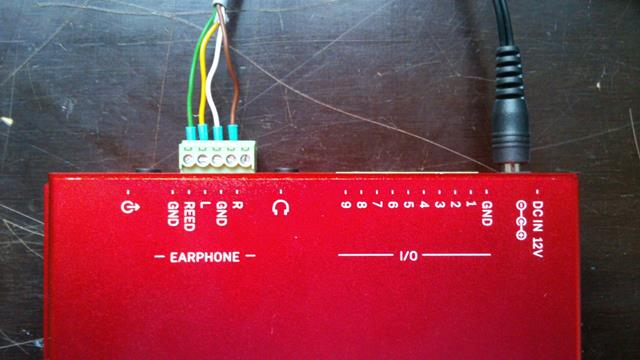
\includegraphics [width=1\textwidth]{images/AP01_Wiring_Detail.jpg}
    \caption{Verkabelung des Mediaplayers}
    \label{verkabelung_mediaplayer}
\end{figure}

\paragraph{Software \& Einstellungen}


\subsection{iPads}

\paragraph{Hardware \& Verkabelung}

\paragraph{Software \& Einstellungen}


\subsection{Machine Learning Stationen}

\paragraph{Hardware \& Verkabelung}

\paragraph{Software \& Einstellungen}



\subsection{CPU}

\paragraph{Hardware \& Verkabelung}

Rechner $\rightarrow$ Strom
        $\rightarrow$ 4x Monitoranschluss (1x HDMI + 3x Displayport + Adapter (?))

\paragraph{Software \& Einstellungen}

Rechner $\rightarrow$ Server für iPads
        $\rightarrow$ Resolume


\newpage
\section{Raum 3 ('Server')}

\subsection{Medizinquiz}

\paragraph{Hardware \& Verkabelung}

\paragraph{Software \& Einstellungen}



\newpage
\section{Raum 4 ('Cloud')}

\subsection{Chatbot 'Aski'}

\subsubsection{Hardware}

\begin{itemize}
\item 5 Surface Pro 6
\item 5 4k-Fernseher
\item USB-Schlösser
\end{itemize}

\subsubsection{Aufbau}

Die Fernseher und Tablets werden in den Seilen als Paare montiert und per Videokabel (Mini-Display Port auf HDMI, 4k-fähig) verbunden. Die USB-Slots werden mit dem beiliegenden Schloss-System vor ungewünschten Zugriffen geschützt.

\subsubsection{Software}

Die Surfaces stellen ihren Inhalt selbst über einen npm-Server bereit. Dieser kann auf dem Desktop mit einem Rechtsklick $\rightarrow$ 'Mit Windows Powershell ausführen' auf die Datei 'Starte Aski' gestartet werden. Der Inhalt kann dann mit Chrome angezeigt werden, wobei Chrome über die Verknüpfung auf dem Desktop gestartet werden sollte. Dabei muss eine Maus an das Surface angeschlossen sein, um das Anzeigefenster für Chat und Video auf den Fernseher zu bewegen.

\end{document}
